% RGB files are exact local render copies. Gaussian camera depth is re-rendered
% from final PLYs; the reference column is DA-V2(RGB GT), not measured GT depth.
\begin{figure*}[t]
  \centering
  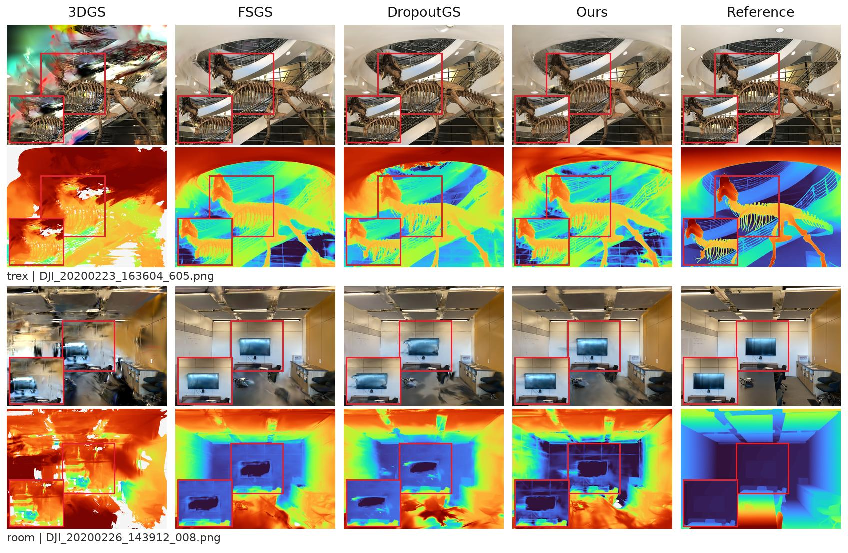
\includegraphics[width=\textwidth]{docs/results_for_paper/figures/llff_rgb_depth_main.pdf}
  \caption{LLFF three-view qualitative comparison at trex and room. Each pair of rows shows RGB and depth at the same held-out camera. Gaussian camera depths share one range per view, determined by the 2nd--98th percentiles of valid full-image depths across methods. The Reference depth is a Depth Anything V2 prediction from RGB ground truth, normalized independently using its 1st--99th percentiles; it is a relative structural reference, not metric ground truth. Warm colors indicate nearer regions. All shown methods use the common MVS initialization and 10k steps. The expanded panel additionally includes CoR-GS and Difix3D+ (30k+30k); DNGaussian remains in the quantitative table.}
  \label{fig:llff_qualitative}
\end{figure*}

\begin{figure*}[t]
  \centering
  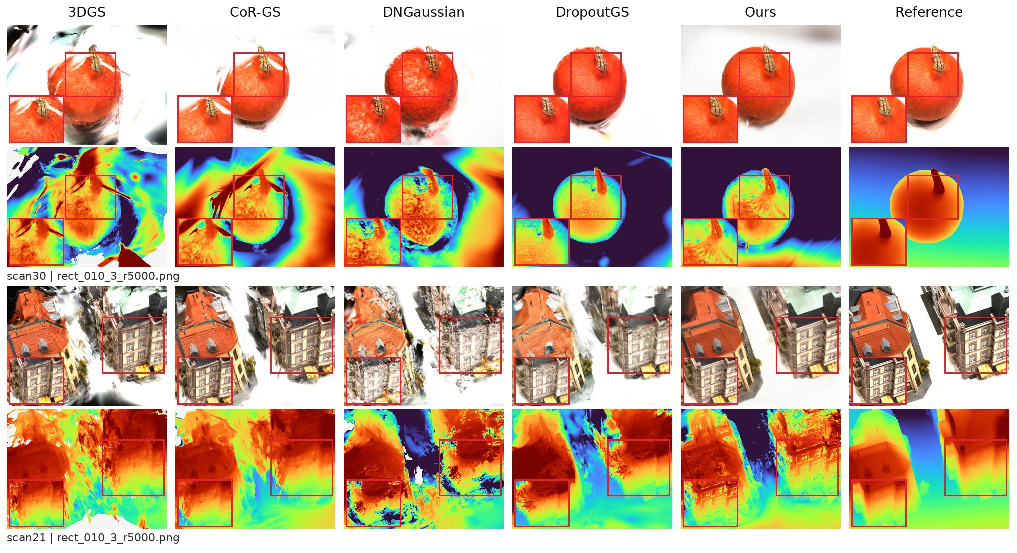
\includegraphics[width=\textwidth]{docs/results_for_paper/figures/dtu_rgb_depth_main.pdf}
  \caption{DTU three-view RGB and depth at scan30 and scan21. Gaussian camera depths share one range per view, determined by the 2nd--98th percentiles of valid depths across methods in the common crop and applied to the full image. The Reference depth is a DA-V2 prediction from RGB ground truth, normalized independently using its 1st--99th percentiles; it is not measured metric depth. Warm colors indicate nearer regions. RGB metrics use the common 25-view object-mask evaluation. DNGaussian and DropoutGS follow the random-point/6k author route; 3DGS, CoR-GS and ours use MVS/10k.}
  \label{fig:dtu_qualitative}
\end{figure*}
